
\documentclass[a4paper,10pt,landscape]{article}
\usepackage{graphicx}
\usepackage{listings}
\usepackage{multicol,multirow}
\usepackage{calc}
\usepackage{ifthen}
\usepackage[landscape]{geometry}
\usepackage[colorlinks=true,citecolor=blue,linkcolor=blue]{hyperref}
\usepackage{sectsty}
\usepackage{mathtools,amsmath,amsfonts}

\ifthenelse{\lengthtest { \paperwidth = 11in}}
    { \geometry{top=.5in,left=.5in,right=.5in,bottom=.5in} }
	{\ifthenelse{ \lengthtest{ \paperwidth = 297mm}}
		{\geometry{top=1cm,left=1cm,right=1cm,bottom=1cm} }
		{\geometry{top=1cm,left=1cm,right=1cm,bottom=1cm} }
	}

\newenvironment{Figure}
  {\par\medskip\noindent\minipage{\linewidth}}
  {\endminipage\par\medskip}
%\usepackage[landscape]{geometry}
\newcommand{\topic}[1]{\begin{center}\section*{#1}\end{center}}

\begin{document}
\begin{center}
     \Large{\textbf{Cheat-sheet Information Retrieval}} \\
\end{center}
\begin{multicols}{3}

\begin{center}
\topic{Term weighting}

\textbf{Law of Zipf}
$frequency\cdot rank = C$
The log lies on a line.

\textbf{Term frequency}
$w_{ij}=tf_i$ frequency of index term i in document j
High frequency content-bearing terms signal main topics in the document 
Terms that occur with a frequency higher than one would expect in a certain passage signal subtopics of the document

\textbf{Inverse document frequency}
$w_{ij} = \log(\frac{N}{n_i})$
Common words that are distributed over numerous texts = poor indicators of a document’s content

Can combine both these: $w_{ij} = tf_i\cdot \log(\frac{N}{n_i})$

\textbf{Length Normalization}
$\frac{tf_i}{\max_{tf_k}}$
Length normalization is used when term frequency is misleading(in documents with different lengths),but not suited when preference to retrieve long documents about a topic.

\textbf{Augmented normalized term frequency}

$\alpha + (1-\alpha)(\frac{tf_i}{\max_{tf_k}})$
Smooth out weights for frequent and infrequent. $\alpha$ usually set to 0.5.

\topic{Retrieval Models}

\textbf{Set-theoretic}
Index terms binary. Queries are conventional boolean expressions in disjunctive normal form.
$Query=  (\neg blue  \land\neg lawyer) \lor car  \lor theft = (0,1,0,1,0) \land(1,1,0,1,0) \land(0,1,0,1,1) \land(1,1,0,1,1) \land(0,1,1,1,1) \land(0,1,1,1,0)$

Similarity 1 if perfect match, 0 otherwise.

Easy to implement but hard to use, and not relative importance or ranking.

Extended Boolean model has documents as vectors in $(0,1)^K$ e.g. (0.1,0.5,1). We get similarities:

$sim(d_j,q_{or})=(\frac{w_{xj}^2+w_{yj}^2}{2})^{\frac{1}{2}}$
$sim(d_j,q_{and})=(\frac{(1-w_{xj})^2+(1-w_{yj})^2}{2})^{\frac{1}{2}} $

\textbf{Algebraic}
Documents and query are represented as term vectors with term weights.

Cosine similarity: $\frac{<q,d>}{\sqrt{<q,q>\cdot<d,d>}}$

Dice similarity:  $\frac{<q,d>}{<q,1>+<d,1>}$

\textbf{Probabilistic}


$P(R=r|D,Q) = \frac{P(D,Q|R=r)P(R=r)}{P(D,Q)}$

We can also use log odds

Classic Model:

$\log\frac{P(D,Q|R=r)P(R=r)}{P(D,Q|R=\Bar{r})P(R=\Bar{r})} = 
\log\frac{P(D|Q,R=r)P(Q|R=r)P(R=r)}{P(D|Q,R=\Bar{r})P(Q|R=\Bar{r})P(R=\Bar{r})} = \log\frac{P(D|Q,R=r)P(R=r|Q)}{P(D|Q,R=\Bar{r})P(R=\Bar{r}|Q)} = \log\frac{P(D|Q,R=r)}{P(D|Q,R=\Bar{r})}+"C" = \log\frac{\prod_iP(D_i|Q,R=r)}{\prod_iP(D_i|Q,R=\Bar{r})}$

Issues: Requires feedback, start will be difficult.

Language Models:

2 assumptions. First is only independent for $\Bar{r}$.

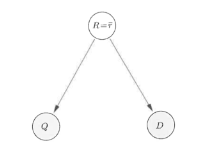
\includegraphics[width=.5\linewidth]{images/LMQD.png}

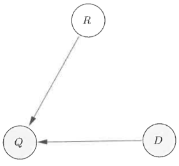
\includegraphics[width=.5\linewidth]{images/LMDR.png}

$\log\frac{P(R=r|Q,D)}{P(R=\Bar{r}|Q,D)} = \log\prod_i^mP(Q_i|D,R=r)+\log\frac{P(R=r|D)}{P(R=\Bar{r}|D)}$ if do second assumption we also get $= \log\prod_i^mP(Q_i|D,R=r)$

LM assumes just one document that generates the query and that the user knows something about this document.

\textbf{Jelinek-Mercer smoothing}

$P(Q|D) = \prod_i(\lambda P_{ML}(q_i|D)+(1-\lambda)P_{ML}(q_i|C))$

(Slides are a bit fucked here)
Simplest estimation is by maximum likelihood:
$P_{ML}(q_i|D) = f(q_i,D)/|D|$,$P_{ML}(q_i|C) = f(q_i,C)/|C|$

How to find value for $\lambda$? EM algorithm!

E-Step:
$m_i = \sum_j^r\frac{\lambda_iP(q_i|RD_j)}{(1-\lambda)P(q_i|C)+\lambda_iP(q_i|RD_j)}$

M-Step:
$\lambda_i =\frac{m_i}{r}$

Where r is the number of relevant documents to a query.
\textbf{Dirichlet smoothing}

$P_{\mu}(q_i|D) = \frac{c(q_i,D)+\mu P(q_i|C)}{|D|+\mu}$

This is equal to Jelinek-Mercer if $\lambda = \frac{\mu}{\mu+|D|}$

We can translate the documents(content pattern) into a conceptual term:

$P(cq_1,...,cq_m|D) = \prod_i(\alpha\sum_lP(cq_i|w_l)P(w_l|D)+\beta P(cq_i|D)+(1-\alpha-\beta)P(cq_i|C))$

We can also add a language model for the query:

Define $\theta_Q \& \theta_D$ as the language models of the query and a document.
Relevance is computed as 

$KL(\theta_Q||\theta_D) = \sum_w P(w|Q)\log\frac{P(w|Q)}{P(w|D)}$ or
$H(\theta_Q||\theta_D) = -\sum_w P(w|Q)\log P(w|D)$ 

{\Large \textbf{LSI - Latent Semantic Indexing} \par}
\end{center}

A term document matrix $A_{txd}$ can be decomposed using SVD to:
$A = U\Sigma V^T$
We can see that $\Sigma^{-1}U^TA = V^T$, it therefore seems reasonable to define: $L = U_k\Sigma_k^{-1}$
If lets pretend that $d_i$ is a column of A
Then we can compare documents in the latent space
$sim(d_i,q) = \cos(L^Td_j,L^Tq)$ \\



\begin{center}
{\Large \textbf{pLSA} \par}
\end{center}

Uses 
\begin{Figure}
    \centering
    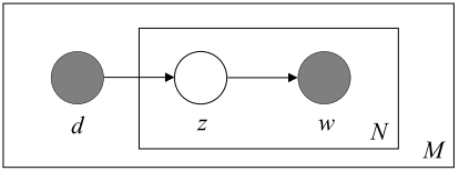
\includegraphics[width=\linewidth]{images/pLSA.png}
    \label{fig:my_label}
\end{Figure}
\begin{Figure}
    \centering
    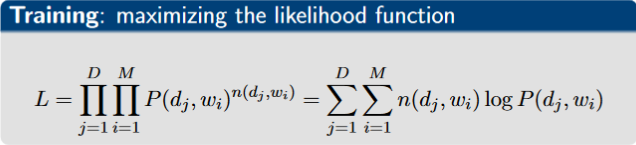
\includegraphics[width=\linewidth]{images/pLSATrain.png}
    \label{fig:my_label}
\end{Figure}
where $n(d_j,w_i) =$ frequency of $w_i\text{ in } d_j$. This is trained with e.g. EM. 

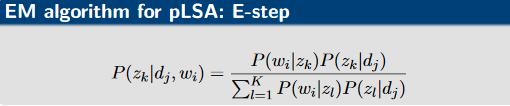
\includegraphics[width=.75\linewidth]{images/pLSAE.png}

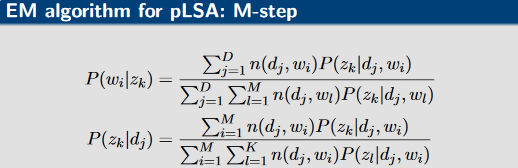
\includegraphics[width=.75\linewidth]{images/pLSAM.png}

\begin{center}
{\Large \textbf{LDA - Latent Dirichlet Allocation} \par}
\end{center}

\begin{Figure}
    \centering
    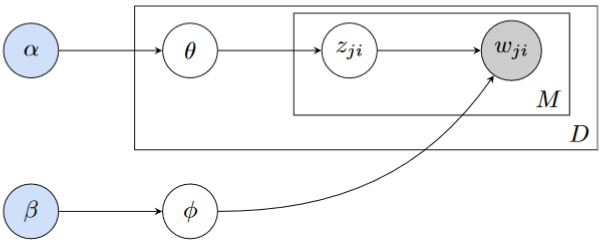
\includegraphics[width=\linewidth]{images/LDA.png}
    \label{fig:my_label}
\end{Figure}

\textbf{Conjugacy of prior:}

Conjugate if $P(X|\theta) \sim A \land P(\theta) \sim B \land P(\theta|X)\sim B$
In our case $z$  is multinomial, therefore the posterior for $\theta$ must be dirichlet (since the prior is also dirichlet).

\textbf{Setting priors}

Good values $\alpha_i = 50/K \beta_i=200/V$

\textbf{Gibbs Sampling}

We fix everything, update the probabilities for z according to:
\begin{equation*}
    P(z_{ji}=k|z_{¬ji},w,\alpha,\beta)\propto \frac{n_{j,k,\negi}+\alpha}{n_{j,k,\negi}+K\alpha}\cdot\frac{v_{k,w_{ji},\neg}+\beta}{v_{k,\neg}+V\beta}
\end{equation*}
Once burned in, sample for each $z_{ji}$. Estimate theta and phi using the below equation.

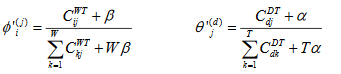
\includegraphics[width=\linewidth]{images/thetaphi.png}

\textbf{Dirichlet}

$\frac{\prod_i \Gamma(\alpha_i)}{ \Gamma(\sum_i(\alpha_i)}\prod_ix_i^{\alpha_i-1}$

\textbf{Multinomial}

$\frac{\Gamma(\sum_ix_i+1)}{\prod_i\Gamma(x_i+1)}\prod_ip_i^{x_i}$

\begin{center}
{\Large \textbf{Word Embeddings} \par}
\end{center}

\textbf{CBOW}
Input is words around word to be predicted, trains hidden weight layer.

\textbf{Skip-gram NNLM}
Input current word, predicts surrounding words.
More expensive since need additional weights and softmax.
Basic formulation is:
\begin{equation*}
    p(w_O|w_I) = \frac{exp(v'_{w_O}^Tv_{w_I})}{\sum_{w=1}^{W}exp(v'_{w_O}^Tv_{w_I})}
\end{equation*}
The sum is very expensive, instead negative sampling is used where only a few of the other words are used. Also importance sampling is used: $P(w_i)=1-\sqrt{\frac{t}{f(w_i}}$ where $t\approx10^{-5}$
\vspace{18mm} 
\begin{center}

\topic{Multimedia Information Retrieval}

Segment images based on local similarity. Videos can be segmented by shot breaks, camera motion, auditory queues textual topic segmentation or multimodal segmentation.

Indexing for images can be done by recognizing patterns, SIFT,CNN, concepts. Same for video as for images.
For audio indexing can be done with speech recognition and transcriping, or from features obtained by deep learning.

{\Large \textbf{Media Information Fusion} \par}
\end{center}

\textbf{Early Fusion}

Feature level multimodal fusion, e.g. combined vector representation of text features, visual features, metadata

\textbf{Late fusion}

Decision level multimodal fusion, e.g. releveance is computed per modality and relevance scores are combined

\textbf{Hybrid fusion}

-

\textbf{Example - Web Search of Fashion Items with Multimodal Querying Laenen et al. 2018}

Query with image and text that alters context of image.
Text is filtered to only related to textual fashion attributes which gives text fragments.
Generate 7 image fragments by exploiting where fashion is found (model images have certain structure). These fragments are represented by CNN features.
Both are mapped to a joint space, image features linearly and words non-linearly.
The objective function is
$C(\theta) = C_F(\theta)+\gamma C_g(\theta)+\beta C_I(\theta)+\alpha ||\theta||_2^2$
$C_F$ measures semantic similarity between all image and text fragments, related to their inner products. We want to maximize inner product for similar semantics and minimize otherwise.
$C_G$ encourages corresponding image text pairs to have a a higher joint similarity compared to other words/ other images.
$C_I$ encourages similar image fragments to correlate to similar text fragments.

\topic{Web Information Retrieval}

\textbf{Crawlers}

Problems: Very large volumes, unstructured data, volatile, redundant

Solution: Crawlers traverse web sending new/updated pages to indexing

Distributed crawling: \textbf{Firewall mode} low coverage \textbf{Cross-over mode} can go into other territories, may duplicate pages \textbf{Exchange mode} Crawlers communicate, gives overhead.

Incremental crawling: Use knowledge of structure of the web to visit sites most likely to have changed since last crawl and record changes

Mirror sites: Crawlers should avoid going to replicas of others sites, for example by URL similarity, link structure, content similarity.

\textbf{Indexing}

Contains important information about the site. e.g. nl index terms and metadata, links, file names, image descriptors etc.

\topic{Indexing Structures}

\textbf{Inverted files}

Index term: Stemmed word, or descriptor

Pointers to documents where index occurs.

Usually triplet $<d,f,[o_1,....,o]>$ where d is the indetifier, f is the frequence and o is the occurance.

Space requirement: \textbf{Heaps' law} vocabulary size grows $O(n^{\beta})$ where $\beta$ around 0.5.

\textbf{Semantic Hashing}

Want to hash to binary code. Difficult for cross modal. Use deep semantic hashing to embedd both modalities.

\topic{Retrieval models}

\textbf{PageRank}

Two ways to approach: $P(p) = (1-\gamma)+\gamma\sum_{d->p}\frac{P(d)}{out(d)}$ or in matrix form $((1-\gamma)U + \gamma M)^T$, where the principal right eigenvector of this equation is the pagerank.
If we add the term $\gamma(\sum_{\in\Gamma}\frac{P(s)}{N})$ for sink nodes, i.e. nodes with only incoming links problems arising from those nodes are lessened.

Personalized: It is possible to show that we can form a personal pagerank by a linear combination of topic pagerank vectors.

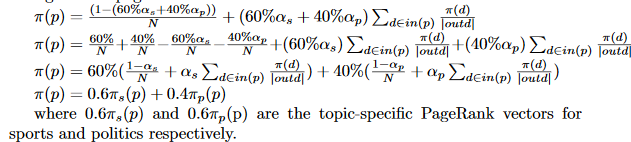
\includegraphics[width=\linewidth]{images/pagerank.png}

\textbf{HITS}

Based on "authority".
High authority if linked from pages with high "hub" weight, hub weights are determined by links to authoritive pages.
Difference from PageRank: We have seperated into authority and hub weights from only 1 weight previously.

\topic{Evaluation Metrics}

\textbf{Recall & Precision}

Recall: Proportion of the relevant documents we can "remember"

Precision: Proportion of documents we retrieve that are relevant

R-precision: Precision(or recall) at Rth position, where R = num. relevant documents

Breakeven point: Recall == Precision

\textbf{F-measure}

$F = \frac{(\beta^2+1)precision \cdot recall}{\beta^2precision + recall}$

\textbf{Non-interpolated average precision(AP)}

$$AP = \frac{1}{|\text{Rel}|}\sum_{r=1}^{|\text{Rel}|}P_r$$
$P_r=\frac{|Arel_r|}{|A_r|}$
When averaged over queries $\xrightarrow{}$ mean average precision(MAP)
Useful for rankings since we care more about the top elements being correct.
Important: We only count precision at points where there is a relevant document!

\textbf{Kendalls $\tau$}

Given a ranking enumerate all pairs. e.g.
$(a,b,c) (b,c,a)$ has 3 pairs $(a,b),(a,c),(b,c)$ in this case $(b,c)$ is the only that agree so: $\tau = \frac{1-2}{3}$ 

\textbf{ROCArea}

$ROC(p,\hat{p}) = \frac{1}{rel(|C|-rel)}\sum_{i:p_i=1}\sum_{j:p_j=0}\textbf{1}_{\hat{p}_i>\hat{p_j}}$

\textbf{Discounted cumulative gain (DCG)}
$$DCG_r = rel_l + \sum_{i=2}^{r}\frac{rel_i}{log_2(i)}$$
Here $rel_i$ is the \textit{graded relevance level} or binary relevance of the document retrieval at rank i.
Question: Why would we put the same weight for the second element and the first? Doesn't seem to make sense to me.

Graded relevance level:
E.g. 6 pt scale from bad to perfect $[0,5]$.
Often used in web search evaluations.

\textbf{Mean Reciprocal Answer Rank (MRAR)}

$MRAR = \frac{1}{n}(\sum_{i=1}^{n}\frac{1}{rank_i}$

where $rank_i = 1,...,\alpha$ where the rank is the first answer in the list that is relevant/correct and n is the number of queries.

\textbf{Depth Pooling}

Union of top k documents retrieved by each system corresponding to a given query is built. Documents in this pool are judged for relevancy with respect to the query.

\textbf{Intrinsic/Extrinsic evaluation}
Compare the answers to answers of expert is intrinsic. How result affects completion of other task completion of other task is extrinsic.

\textbf{WUPS score (probably only relevant for 6pts)}
$W(A,T) = \frac{1}{N} \sum_{i=1}^{N}min[\prod_{a}max_tsim(a,t),\prod_tmax_asim(a,t)]$

Basically for each answer word we multiply the maximum similarity to any ground truth answer and same for the opposite and then we take the minimum.

Ex:
Consider A = {a,b} , T = {a,b,c}(N=1)
$W(A,T) = min(1*1,1*1*sim(b,c))=sim(b,c)$
Where the similarity is probably less than 1. I don't personally understand why there is a multiplication and not just averaging, but perhaps there is some good reason, I suppose it more heavily punishes if several words are not exactly correct, e.g. if one word has 0.5 similarity and the rest 1 the punishment is less than if all of them have 0.8.

\topic{Types of clusterings}
Sequential - One pass through data, assign to clusters , Hierarchical - Either build up clusters by merging or split clusters, Cost function optimization - Try to optimize cost functions of clusters based on assignments. 
\topic{Hierarchical Clustering}
Either bottom up or top down. \textit{Agglomerative} means bottom up and \textit{Divisive} means top down.
Clusters are sometimes represented by centriod (not a real object), or representative(e.g. object closest to centriod) object of cluster.

\textbf{Agglomerative}:

Start with singleton clusters. At each timestep merge the 2 most "similar" cluster pairs based on \textit{proximity function}.
Different proximity functions:
\textbf{Single linkage}: Shortest distance between clusters
\textbf{Complete linkage}: Farthest distance between clusters
\textbf{Group average linkage}: Average distance, efficient if using a "mean vector"

\textbf{Objective function}

K-means

Non-negative Matrix Factorization(NMF): Find $A=UV$ such that all $u,v>0$ and minimize some cost function. E.g. squared error or KL-divergence. If trained by KL-divergence it is equivalent to pLSA. Can also view as U means terms to clusters and V as documents to cluster.

\topic{Classification }
\textbf{Feature selection}
Which features are relevant for classification? Can use frequent item sets(e.g. with apriori) , unigrams hypercliques(correlation of features).
Can also use supervised selction, for example
\textbf{$\chi^2$ measure:} Measures the degree of dependence (lack of independence) between an observed probability distribution and an expected distribution.

Definition: $\chi^2(f,c)=\frac{n(n_{++}n_{--}-n_{-+}n_{+-})^2}{n_{c}n_{\sim c}n_{f}n_{\sim f}}$

\textbf{Feature extraction}
E.g. LSI,LDA, word embeddings, word2vec,BERT, or from supervised learning, (often referred to as representation learning)
\textbf{ML-algorithms}
\textbf{NB}:
$P(C|D) =  \frac{P(D|C)P(C)}{P(D)} = \frac{P(D|C)P(C)}{P(D|C)+P(D|\neg C} $ Here the assumtion is that all the data is independent given the class, so $P(D|C)$ is "easy" to calculate. MNB is simply Multinomial Naive Bayes. Fast results!

\textbf{SVM}:
$ min |w|^2 \text{ with } y_i(<w,x_i>+b) - 1 \geq 0$
We can instead solve the dual system, using the Lagrange Duality the dual system is 
$\sum_i\lambda -\frac{1}{2}\sum_{i,j}\lambda_i\lambda_jy_iy_j<x_i,x_j>$
$s.t \lambda > 0 && \sum_i\lambda_iy_i = 0

\textbf{kNN}
Important to have good discriminatory features and similarity metrics/kernels. \textit{Metric learning} deals with finding similarity function between examples.

\textbf{Hierarchical classification}

Flat classifiers trains 1 classifier to predict leaf nodes.

Local classifiers: Train classifiers on part of some tree structure
\begin{Figure}
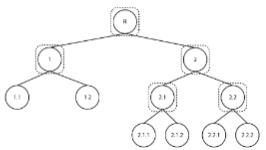
\includegraphics[width=.5\linewidth]{images/hierarchy.png}
\end{Figure}
We predict greedily down the DAG. Possible to use different features at each classifier. Can combine prediction by traversing more branches.
 
 Issues:
 Errors high up cannot be recovered.
 Higher nodes are more complex
 Few training examples low down in hierarchy.
 
 Solutions:
 Refinement - Extend features with predictions of lower children.

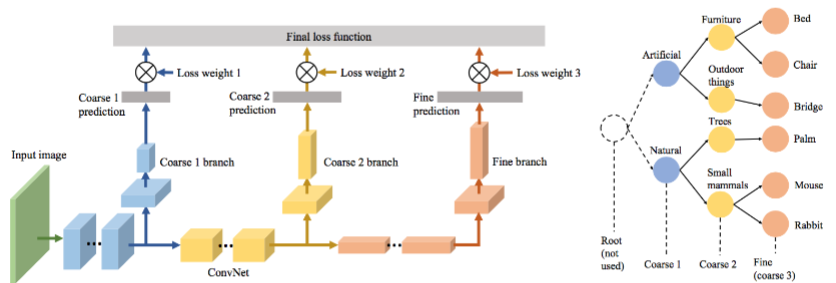
\includegraphics[width=\linewidth]{images/CNN_hierarchy}

\textbf{Extreme classificiation}
Millions of labels. Need fast training and prediction.

 Example: Slice
 
 Learns one linear classifier per label, but reduces costs per num labels to from N to log(N). Intuition: only small number of labels active in a given region of the feature space. For testing approximate NN is used to find the proper classifiers.
 
 \topic{Information Extraction}
 Important part of IR.
 
 Difficulties:
 
 How to cope with limited data
 
 Reducing feature engineering - Deep Learning
 
 \textbf{IE kernels}
 
 \textbf{String subsequence kernel(SSK)}:
 
 All (non-contiguous included) substrings of n-symbols. 
 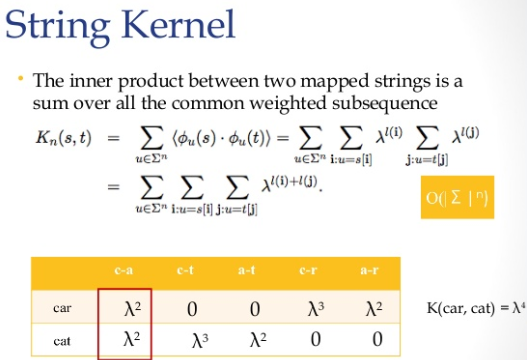
\includegraphics[width=\linewidth]{images/stringkernel.png}
 Here the subsequence kernel counts all subsequences that are shared between the strings, and weights them by their lengths. In the slides the kernel is defined as:
 $\sum_n^N K_n(s,t,\lambda)$
 
 \textbf{Relational kernel}:
 
 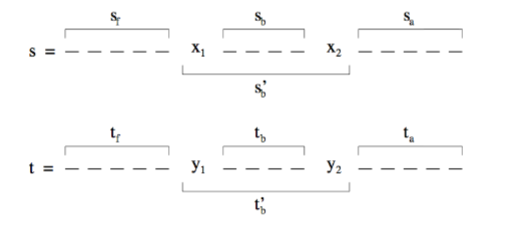
\includegraphics[width=\linewidth]{images/relationalkernel.png}
 
 $rK(s,t) = K^{fb} +  K^b + K^{ba}$
 $K^{fb}(s,t)$ =  number of common fore-between pairs in segment spanned by “fore”(sf, tf) +  “between”(sb, tb) entities (x1,y1) and (x2,y2) included, i.e., (sb’, tb’ )
 
 $K^{b}(s,t)$ = number of common between pairs in segment spanned by (sb’, tb’) 
 
 $K^{ba}(s,t)$ = number of common between-after pairs in segment spanned by (sb’, tb’) +  “after”(sa, ta)

\topic{Compression in IR - 6 study points}

\textbf{Zero-order models}: The probabilities are independent

\textbf{Prefix-free}: There is no code word as prefix for another code word

\textbf{Huffman coding}

Algorithm:
For each symbol create node. Merge the nodes with smallest probablities iteratively.

Time complexity: $O(n\log(n))$

Variants - Byte Huffman:

Bytes as symbols of the target alphabet.

Can also have tagget/end-tagged huffman bytecode where first bit indicates if first byte of codeword. These are faster but a bit less compression.

\textbf{Compressing postings lists}

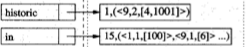
\includegraphics[width=.5\linewidth]{images/invertedfile}

We convert to $\Delta$-values. i.e. difference between neighbouring positions.
Methods

\begin{itemize}
\item Nonparametric codes - static, do not take into account $\Delta$ distribution e.g. $\gamma$ -code
\item Parametric codes - semi-static, take advantage of the distribution.
\end{itemize}


\textbf{$\gamma$ -code}

2 components: Selector \& body.

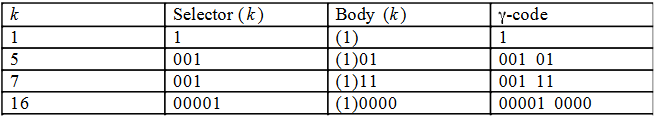
\includegraphics[width=.75\linewidth]{images/gammacode.png}

Selector describes the length of the body by 0s ended by a 1.

\textbf{$\delta$-code}

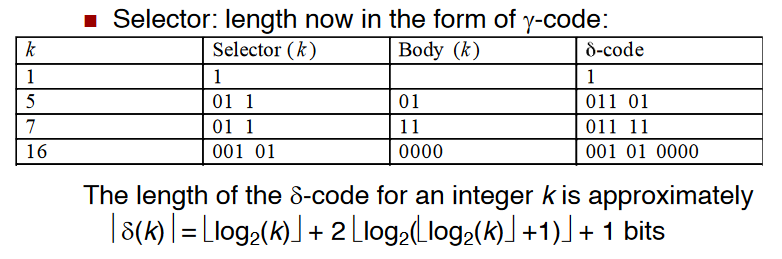
\includegraphics[width=.75\linewidth]{images/deltacode.png}

Uses a $\gamma$ -code for the selector, better for long codewords.

\textbf{$\omega$ -code}

Encoding:
\begin{lstlisting}
code = 0
while N != 1
    code = [bin(N) code]
    N = len(bin(N))-1
\end{lstlisting}

Decoding:
\begin{lstlisting}
N = 1
ind = 0
while code[ind] != 1
    N = code[ind:ind+N]//Inclusive
    ind += N+1
\end{lstlisting}

\textbf{Golomb/Rice codes}

Encode:

Choose M:

q,r = floordiv(N/M), mod(N,M)

code = unary(q)+0 //I.e. 3 = 111 0

code += truncated bin(r)

Truncated binary:

b = len(bin(M))

if $r < 2^b-M$

    use b-1 bits to encode

else

    use b bits to encode

\textbf{LLRUN}

Huffman codes are difficult to use because the set of distinct gaps is about the same as the number of documents. Since the huffman tree needs to store all the distinct gaps it doesn't really reduce size.

Instead we store all gaps in buckets like:
$B_j = [2^j,2^{j+1}-1]$ used as selector, then j-bit body.

\textbf{Interpolative coding}
$L = (2,9,12,14,19,21,31,32,33)$
Encode first and last using e.g. $\gamma$-code. $L[5] \in [6,29]$. Then recursively divide and conquer.

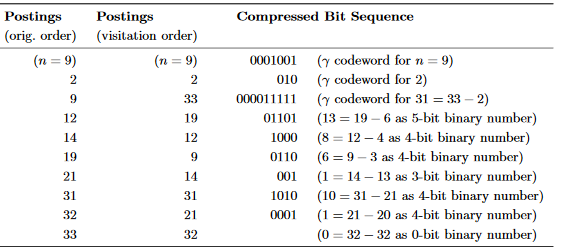
\includegraphics[width=\linewidth]{images/interpolative.png}

\textbf{Byte aligned codes}
Easiest way: Split $\Delta$-value into 7 bit chucks and prepend with a flag bit indicating end of sequence.

\textbf{Word aligned codes}
Simple-9: Reserve first 4 bits(selector) to indicate 9 different kinds of splits. See below:

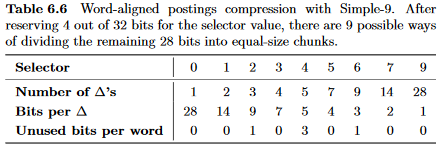
\includegraphics[width=\linewidth]{images/simple9.png}

\textbf{Decoding unaligned codes}
If length of gaps is known we can have a table lookup for b bits instead of 1 bit sequential.

\textbf{Dictionary Compression}

Group consecutive terms and use pointers to start and end. Front coding:
〈“shakespeare”,(11,2,“an”),(13,3,“ism”)
Lempel-Ziv coding after front coding. We can also interleave dictionary with postings.

\topic{Learning to Rank - 6pts only}

\textbf{Loss functions}

Hinge-loss: $L(y,\hat{y}) = \max{0,1-y\hat{y}}$
Exponential loss: $L(y,\hat{y}) = e^{-y\hat{y}}$
Logistic loss: $L(y,\hat{y}) = \log{1+e^{y\hat{y}}}$

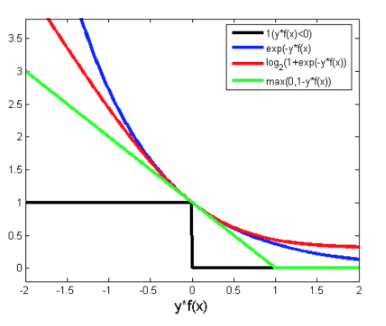
\includegraphics[width=.75\linewidth]{images/rankloss.png}

\textbf{Pointwise approach}

Input: Feature vector for each document

Output: Score: relevance degree or class that represents relevancy

Loss: Usually mean squared error(cross entropy for class?)

Assumption: Relevance is absolute: a document is judged independently to the other documents for a given query.

\textbf{Pairwise approach}

Input: Pairs of documents, each document feature vector, or pair is represented as feature vector

Output: Pairwise preferences $\in {1,-1}$, can also be pointwise and then combined i.e. $h(x_u,x_v) = 2(f(x_u)>f(x_v))-1$

Loss: $\text{argmin}_h\sum_q\mathcal{L}(h(x_j^q,x_k^q),y_{j,k}^q$
e.g. pointwise functions then $\text{argmin}_h\sum_q\tau(2(f(x_u)>f(x_v))-1,y_{j,k}^q)$

Kendall's $\tau$ measures pairwise inconsistencies.

Assumptions: No longer assume absolute relevance, classification on document pairs w.r.t. same query.

Example:(\textbf{RankNet}, FRank, RankBoost, Ranking SVM, etc.)

Suppose nn computes scores $s_i = f(x_i^{(q)})$,$s_j = f(x_j^{(q)})$

Probability that "$d_i > d_j$" = $\frac{1}{1+e^{-\sigma(s_i-s_j)}}$, $\sigma$ determines shape of sigmoid.


Let $S_{ij} \in {-1,0,1}$. We can the compare to GT $\Bar{p_{ij}}= (1+S_{ij})/2$

$\mathcal{L} = -\Bar{p_{ij}}\log(p{ij})-(1-\Bar{p_{ij}})\log(1-p_{ij})$

Does not model that errors higher up are worse than lower down! Question: Can't we just weigh the pairs in the loss function depending on the position?

\textbf{Listwise approach}

Input: A set of documents associated with the query

Output: A ranked list (or permutation)

Loss:

$h = argmin_h \sum_q \mathcal{L}(h(x^q),y^q) = e.g. argmin_h \sum_q(1-AP(h(x^q),y^q))$
$SVM^{MAP}$

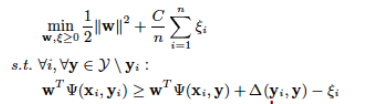
\includegraphics[width=\linewidth]{images/svmmap.png}

Formulated as a structured SVM. $\Psi$ is a joint feature map. For each pair a set of constraints in the form above is added to the optimization, exponential amount. Solved by only solving with respects to the constraints with the highest violations. The constraints with highest violation are find by first sorting the non-relevant and relevant documents by $\theta(x,d_i)$ we use the property that the AP loss is invariant to position changes between relevant or non-relevant documents to reduce the problem to interleaving the two sorted lists. This is solved in O(n) time, which is very nice.

\textbf{RankCosine}

Loss is given by cosine similarity between score vector from scoring function f and query q and the GT score vector:

$\mathcal{L}(f;x,y) = 1/2 - \frac{\sum_j^m\varphi(y_j)\varphi(f(x_j))}{\sqrt{\sum_j^m\varphi(y_j)^2}\sqrt{\sum_j^m\varphi(f(y_j))^2}}$

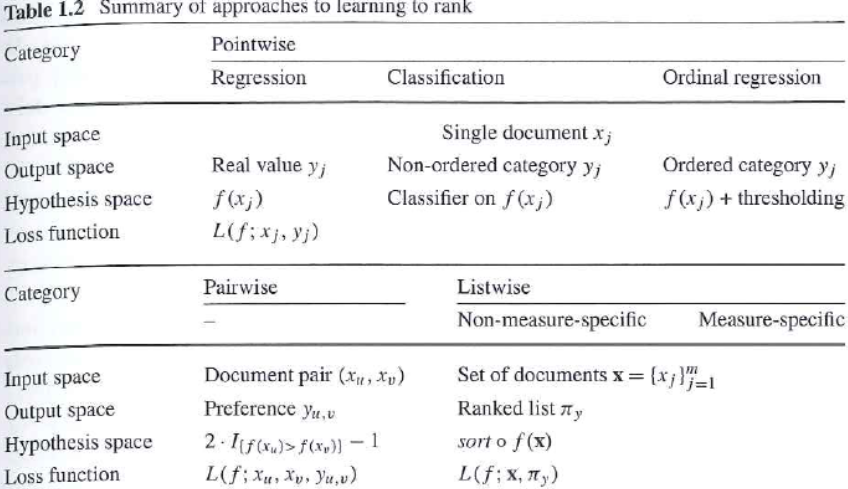
\includegraphics[width=\linewidth]{images/learningtoranksummary.png}

\textbf{Diversity}

\begin{itemize}
    \item Discover information facets of a specific query
    \item Assess relevance of a document to a particular facet
    \item Order results by optimization
\end{itemize}

In some approaches first steps are skips, just add loss function e.g. Maximal Marginal Relevance, maximize implicit user feedback etc.

Can also predict an entire ranking, fits structure prediction models.

Potential development for structured prediction models where relation between documents are important.

\end{multicols}
\end{document}